\section{The DFW Scheduler}
\label{sec:schedulers}

The asynchronous program semantics of the previous section are defined with
respect to an implicit task \emph{scheduler}, which enables any non-completed
task to execute at any time. Computing the reachable global valuations $R(P)$
of arbitrary programs $P$ is costly. One compelling approach for lowering the
cost of program exploration is by considering specialized \emph{delay-bounded}
schedulers with limited nondeterminism~\cite{conf/popl/EmmiQR11}. In this
section, we provide a formal operational characterization of Emmi et al.'s
$K$-delay bounded depth-first scheduler $\df(K)$~\cite{conf/popl/EmmiQR11}, as
well as our novel synchronization-exploiting scheduler $\dfw(K)$.

A \emph{scheduler} $@Y = \tup{Q,q_0,@d,\pi}$ is a set $Q$ of states with
initial state $q_0 \in Q$, a transition function $@d : Q \x ((\<Ids> \x
\<Configs>^2) \U \set{ @e }) -> Q$, and a task-selection predicate $\pi : Q ->
\<Ids>$. Intuitively, a scheduler state $q \in Q$ determines the task $\pi(q)
\in \<Ids>$ that is enabled to make a program transition. A transition
$@d(q,i,c_1,c_2) = q'$ determines the scheduler's successor state $q'$ to a
program transition $c_1 -> c_2$ of enabled task $i$ from scheduler state $q$.
We represent nondeterminism using $@e$-transitions $@d(q,@e)$; these
transitions affect scheduler state only, and not program configuration
otherwise. We say $@Y$ is \emph{deterministic} when $@d(q,@e) = q$ for all $q
\in Q$.

As an example, we could define a completely nondeterministic scheduler
$\tup{Q,q_0,@d,\pi}$, which always enables all pending tasks, with states $Q =
\<Ids>^{*}$ represent scheduling queues, having initial state $q_0 = \nil$; the
task-selection predicate $\pi(i \cdot \_) = i$ selects the task at the head of
the queue. Transitions modify the queue accordingly: enqueueing created tasks
$j$ on {\sc Async} transitions $c_1 -> c_2$, $@d(i\cdot I,i,c_1,c_2) = i \cdot
I\cdot j$; otherwise not modifying the queue, $@d(i \cdot I,\_,\_,\_) = i \cdot
I$; and rotating the queue on $@e$-transitions, $@d(i \cdot j \cdot I,@e) = j
\cdot I \cdot i$. By making a sequence of $@e$-transitions, this scheduler can
enable any previously-created task.

To define the executions admitted by a scheduler $@Y$, we make $@Y$ follow
program transitions, and allow $@Y$ to make $@e$-transitions at any time.
Formally, an \emph{$@Y$-execution} is an execution $c_0 c_1 .. c_j$ such that
there exists a sequence $q_0 q_2 .. q_{j'} \in Q^{*}$ and a monotonic injection
$f : \mathbb{N}^{<j} -> \mathbb{N}^{<j'}$ such that for each transition $c_i ->
c_{i+1}$ of task $u_i$, for $0 \le i < j$, $u_i$ is enabled by $@Y$: $u_i =
\pi(q_{f(i)})$; and the state of $@Y$ follows the transition $c_i -> c_{i+1}$:
$@d(q_{f(i)},u_i,c_i,c_{i+1}) = q_{f(i)+1}$; additionally, intermediate
$@Y$-states follow $@e$-transitions: $q_{i+1} = @d(q_i,@e)$ for $0 \le i < j'$
where $i \notin \<range>(f)$. Finally we define $R(P,@Y)$ as the set of global
valuations reached in finalized $@Y$-executions of $P$.

We define both the $\df(K)$ and $\dfw(K)$ schedulers over states which
represent the ordered tree of tasks of an execution, in which the children of
each node $i$ are the tasks which task $i$ has called asynchronously, in the
order in which they are called. Formally, the \emph{Depth-First
Scheduler}~\cite{conf/popl/EmmiQR11} is the scheduler $\df(K) =
\tup{Q,q_0,@d,\pi}$ such that
\begin{itemize}

  \item[$Q$] is the set of vertex-labeled trees $\tup{V,E,@ll,d}$ with
  vertices $V \subset \<Ids>$, edges $E$, and labeling function $@ll : V ->
  (\set{\mathsf{R},\mathsf{C}} \x \<Nats>)$, assigning each vertex $@ll(i) =
  \tup{b,k}$ a {\sf R}eady or {\sf C}ompleted status $b$ and a round number $k
  \in \<Nats>$, along with a \emph{delay counter} $d \in \<Nats>$.

  \item[$q_0$] is the tree $\tup{\set{\nil},@0,\set{\nil |->
  \tup{\mathsf{R},0}},0}$.

  \item[$\pi(q)$] is the least, in depth-first
  order, minimal-round ready vertex as in Figure~\ref{fig:dfw}(a), 
  and is undefined when $q$ does not contain such a vertex.
    
  \item $@d(q,i,\_,\_)$ is obtained from $q$ for {\sc Async} transitions
  creating task $j$ by adding a rightmost child $(j |-> \tup{\mathsf{R},k})$ to
  the $\tup{\mathsf{R},k}$-labeled vertex $i$, as in Figure~\ref{fig:dfw}(b).
    
  \item $@d(q,i,\_,\_)$ is obtained from $q$ for {\sc Complete} transitions
  by updating $i$'s label from $\tup{\mathsf{R},k}$ to $\tup{\mathsf{C},k}$.
    
  \item $@d(q,i,\_,\_) = q$ otherwise.
  
  \item $@d(q,@e)$ is obtained from $q$ by incrementing the delay counter $d$,
  and updating $\pi(q)$'s label from $\tup{\mathsf{R},k}$ to
  $\tup{\mathsf{R},k+1}$, so long as $d < K$; otherwise $@d(q,@e) = q$.

\end{itemize}
Note that at each step of $@d$, the label of at most one task can change.
Furthermore, $\df(0)$ is deterministic.

\begin{figure}[t]
  \centering
  \begin{minipage}{3cm}
    \centering
    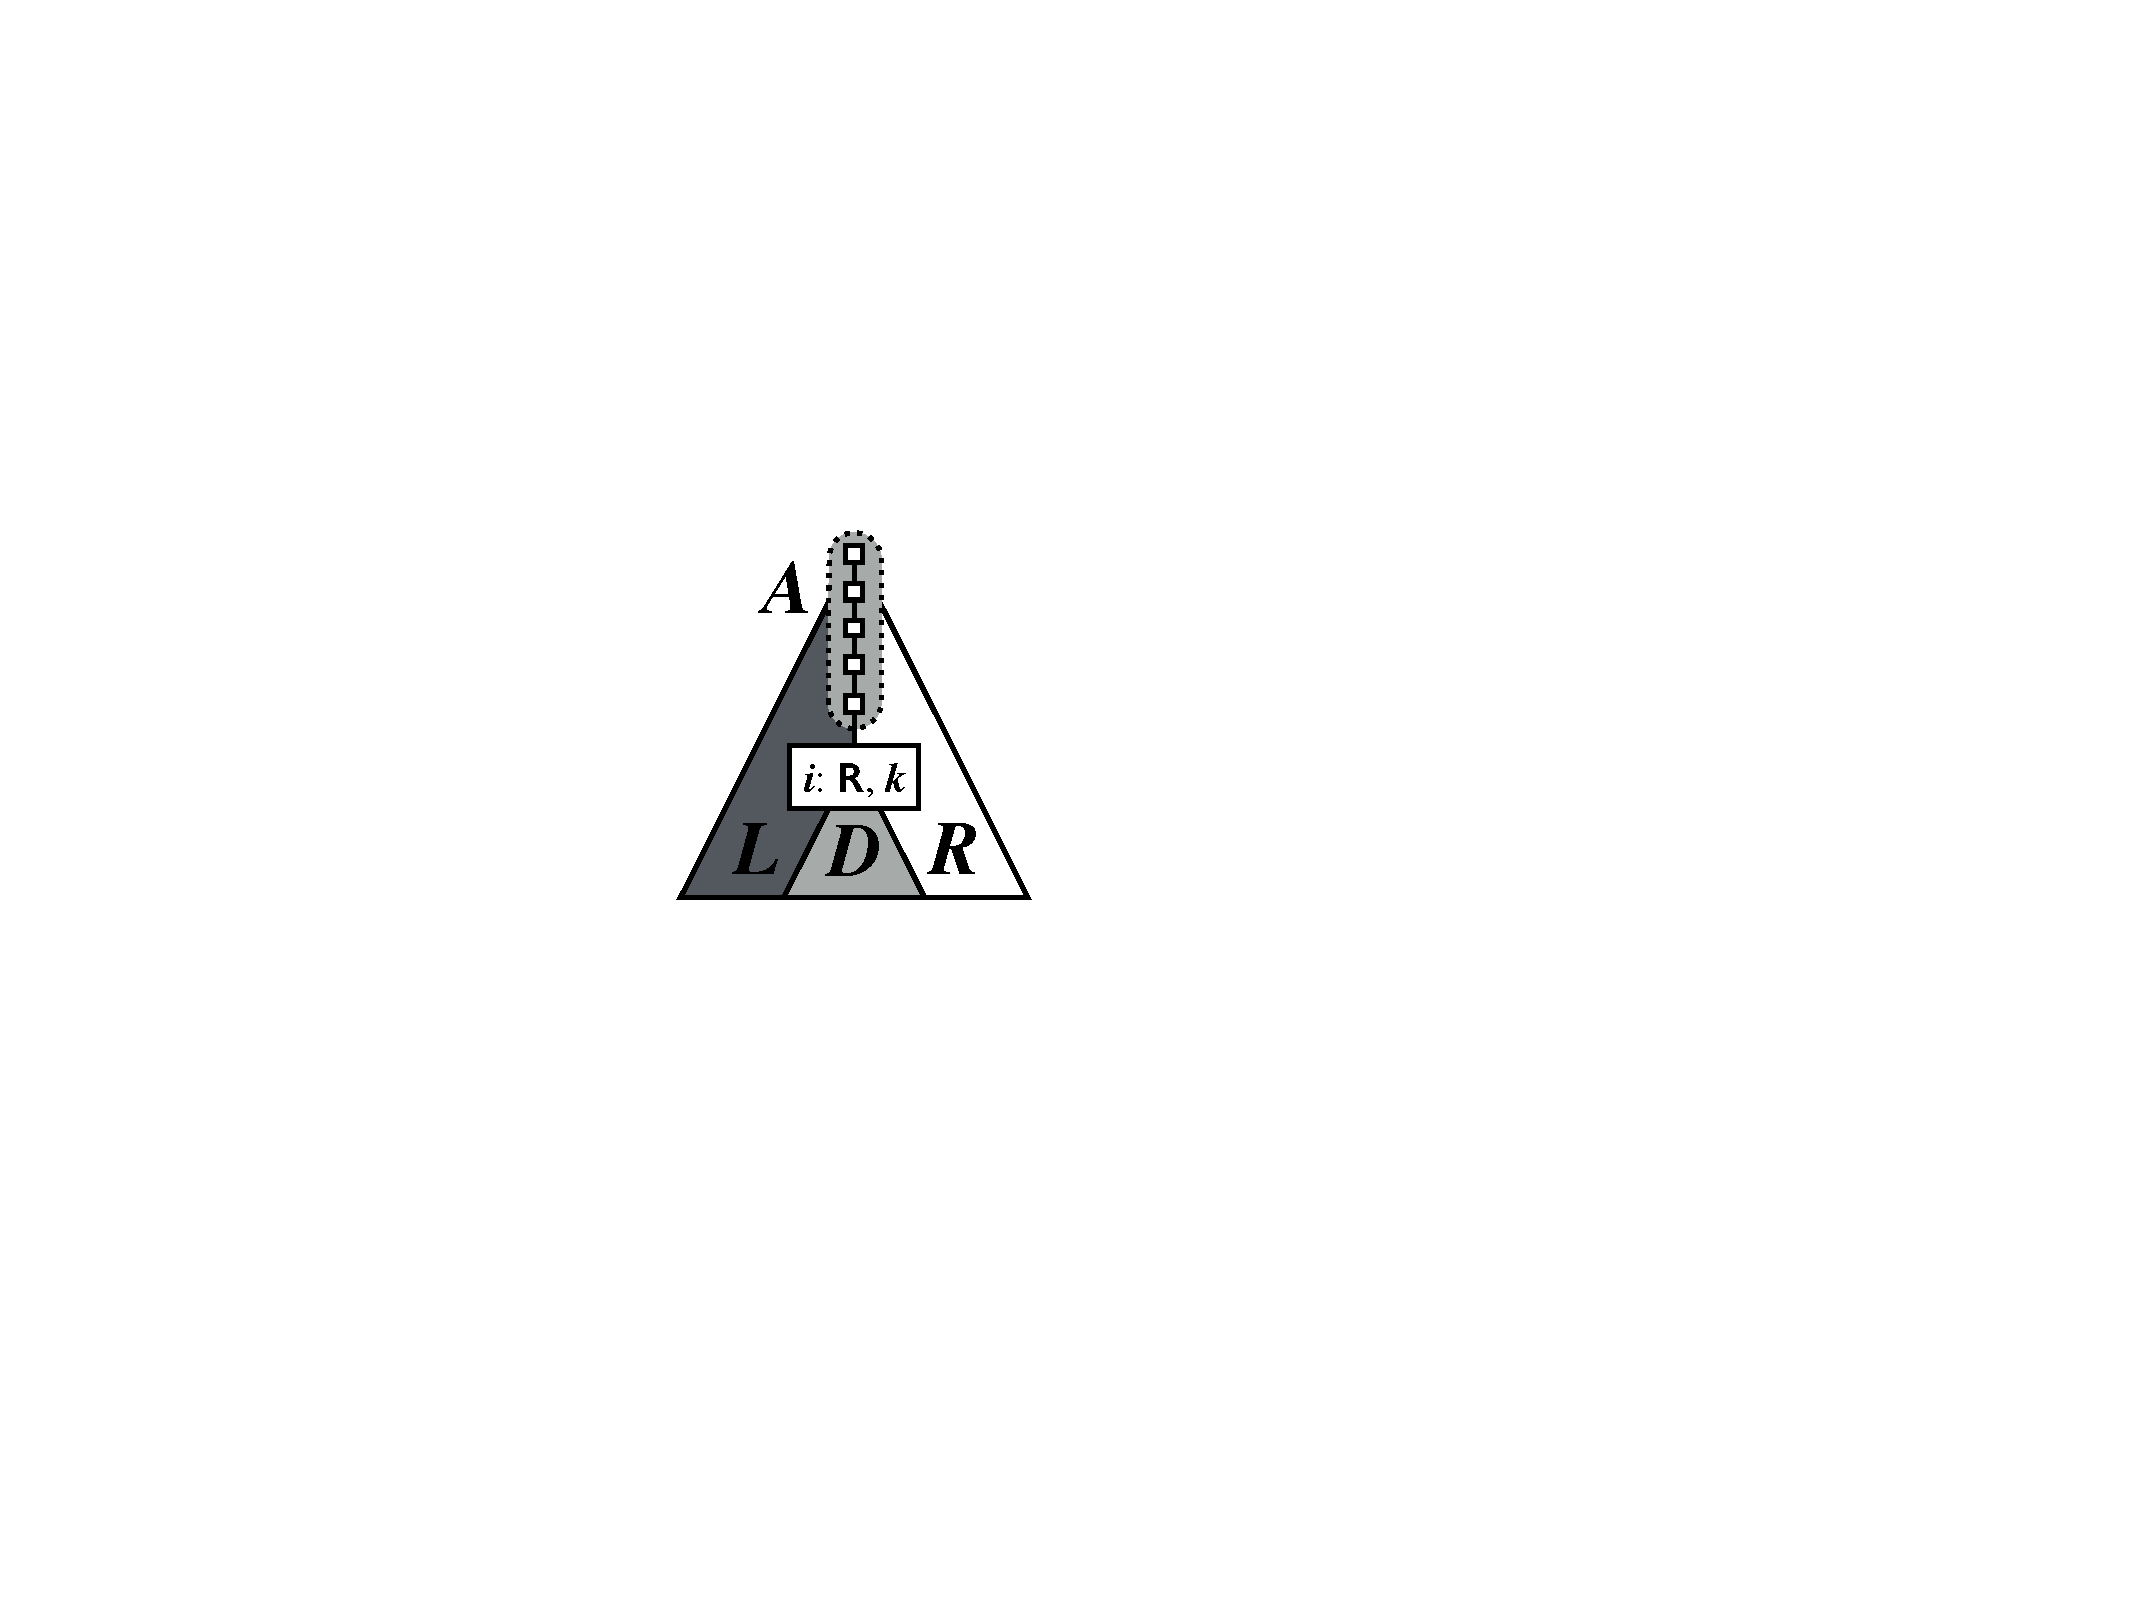
\includegraphics[width=3cm]{figures/figure-dfw-tree}
    (a)
  \end{minipage}
  \hspace{1cm}
  \begin{minipage}{3cm}
    \centering
    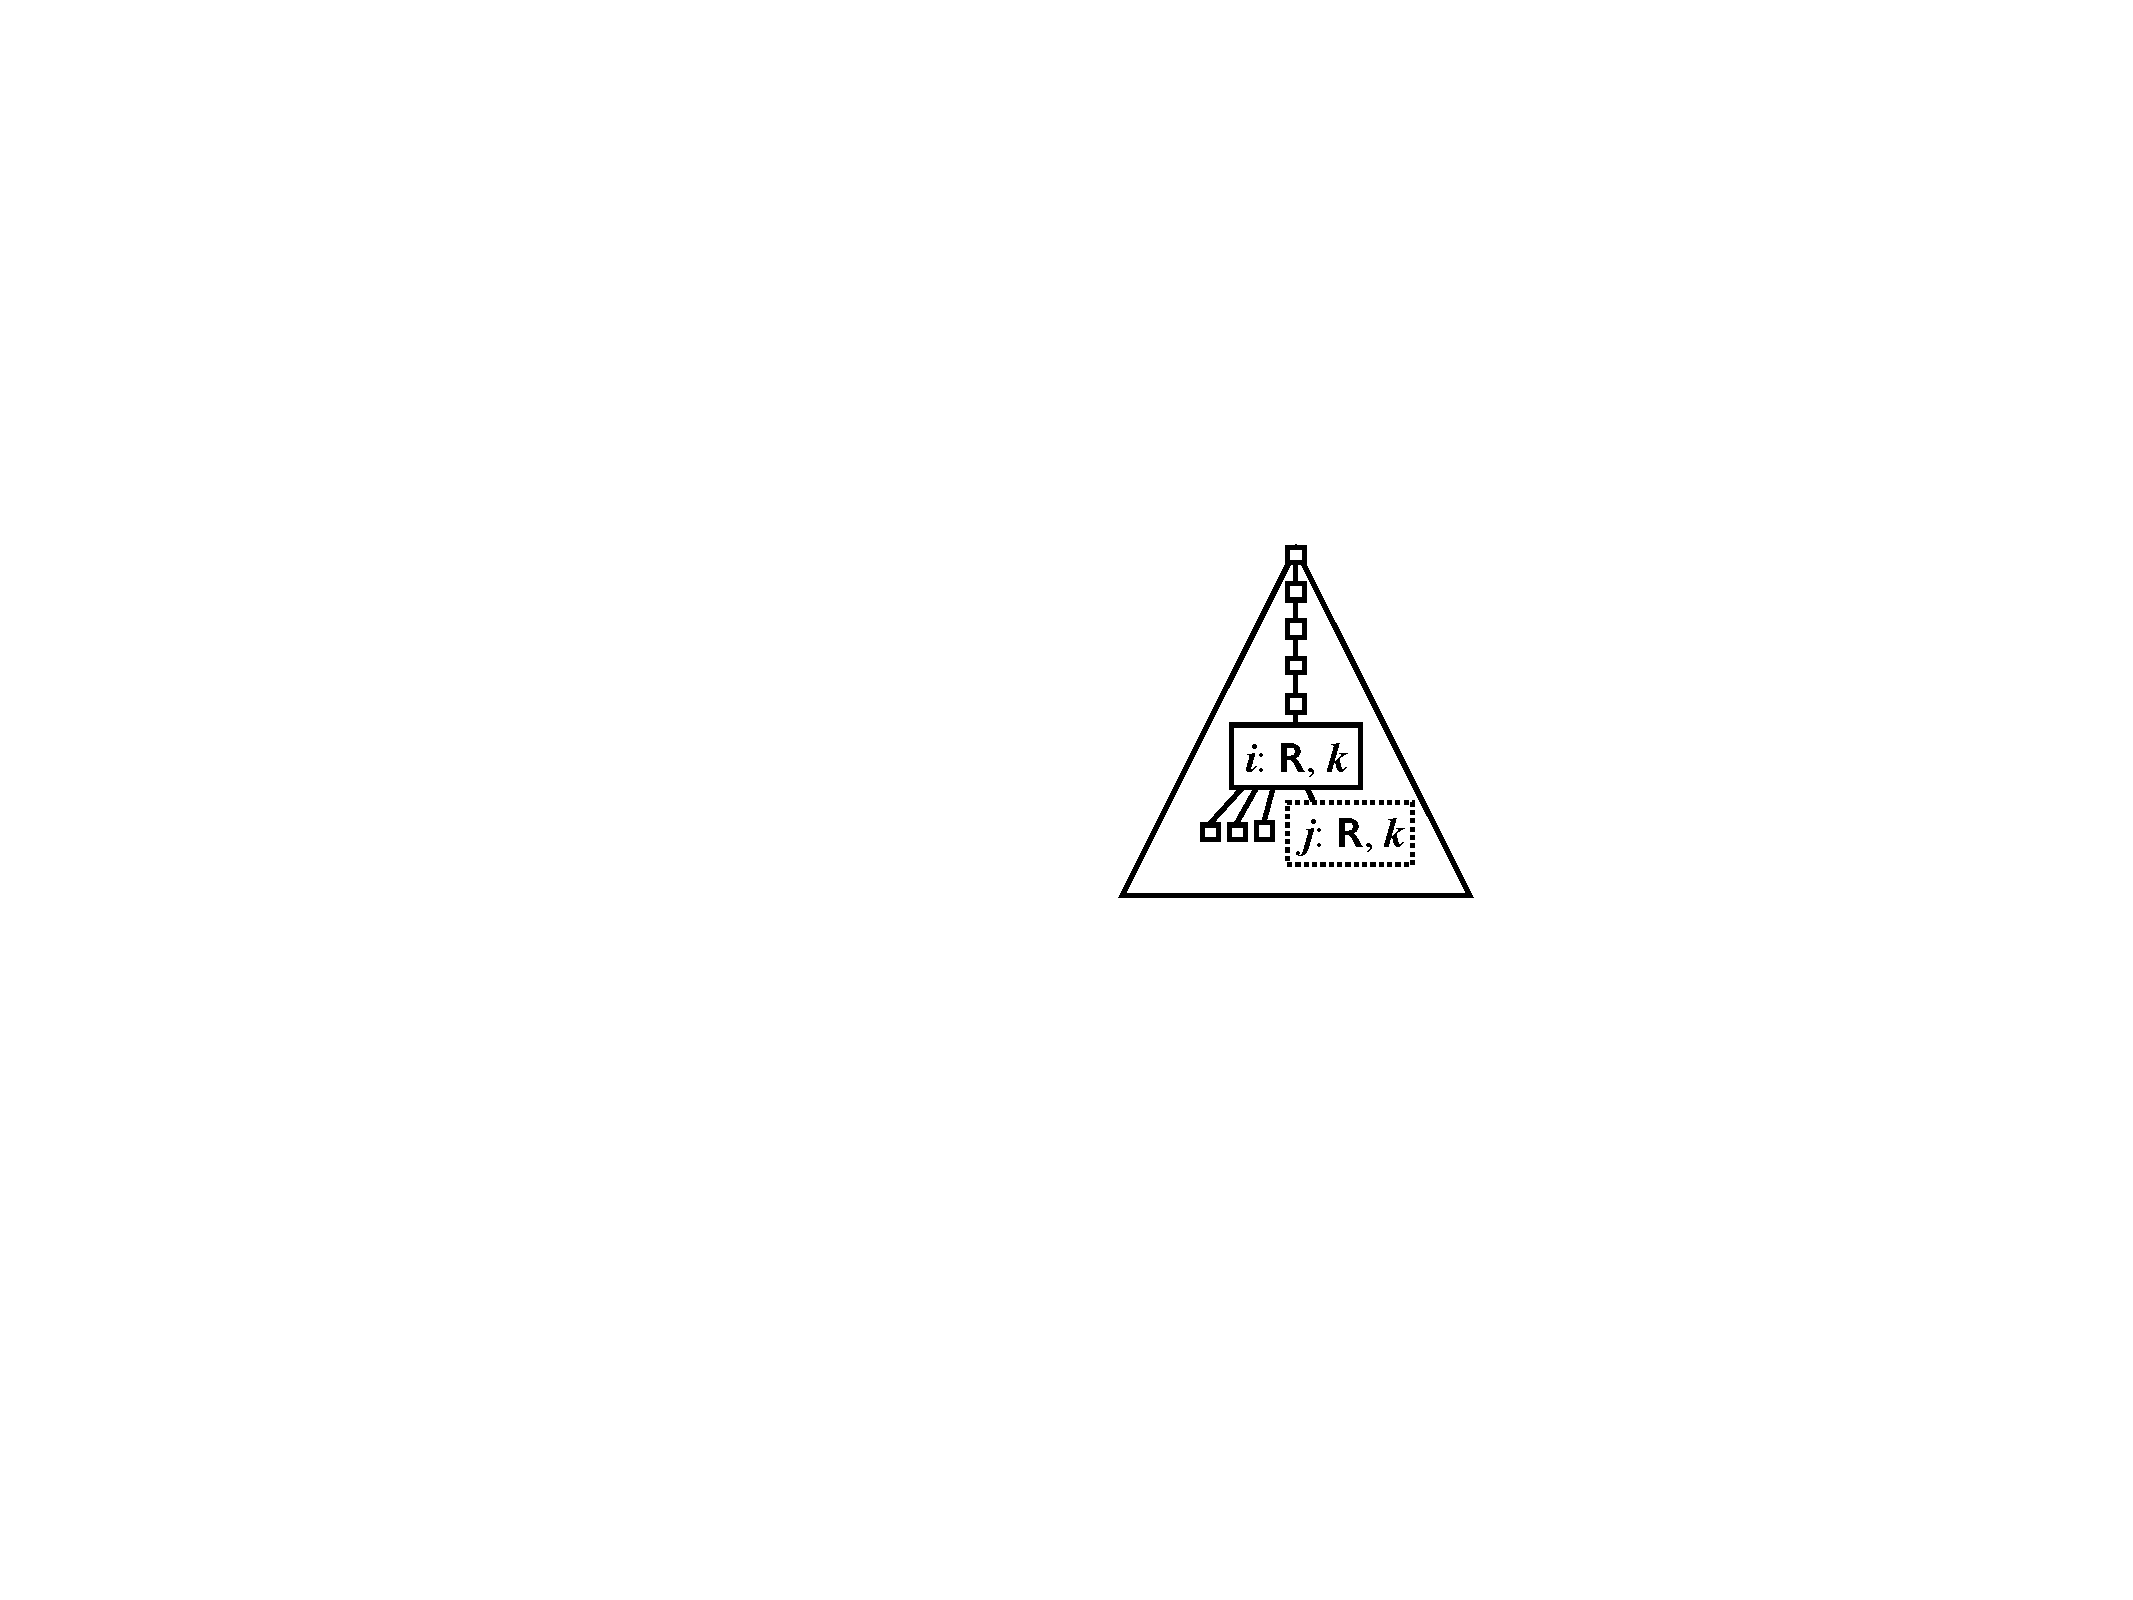
\includegraphics[width=3cm]{figures/figure-dfw-post}
    (b)
  \end{minipage}
  \caption{(a)~A tree of the $\df(K)$ scheduler enabling task $i$,
    showing $i$'s ancestors ($A$), descendants ($D$), and the left ($L$) and
    right ($R$) descendants of $i$'s ancestors.  As $i$ is enabled, each
    node in $A \U L$ is either completed or has round $>k$, and each node
    in $D \U R$ is either completed or has round $\ge k$.
    (b)~When task $i$ posts $j$, $\df(K)$ adds $(j |-> 
    \mathsf{R},k)$ as $i$'s rightmost child.}
  \label{fig:dfw}
\end{figure}

Intuitively, $\df(K)$ keeps track of a notion of execution
\emph{rounds} from $0..K$ over which tasks execute, and executes lowest-round
tasks in depth-first order according to the task tree. For instance,
$\df(0)$ allows only a single round of execution, and executes each
task in depth-first order until either all tasks are completed, or the task
currently enabled by $\df(0)$ blocks. $\df(1)$ executes tasks
according to the same order, except that the execution of one single task can
increment the delay counter, and be postponed to the second round, resuming if
and after which all other tasks complete in the first round. Note that when the
currently enabled task in $\df(K)$ is blocked, execution can only
progress by advancing the blocked task to a subsequent round, and incrementing
the delay counter. As the delay bound $K \in \<Nats>$ is increased, the cost of
exploration can greatly increase, as $\df(K)$ can allow exponentially
more schedules.

To avoid increasing the delay bound $K \in \<Nats>$, which exponentially
increases the number of alternate schedules explored, and ultimately increases
the cost of exploration, we define a scheduler that does not enable tasks that
are blocked waiting for others to complete. We define the
\emph{Synchronization-Exploiting Depth-First Scheduler} $\dfw(K) =
\tup{Q,q_0,@d',\pi}$ by extending $\df(K)$ to label each tree node $i$
with an additional {\sf W}aiting status label, and a counter for the number of
tasks that $i$ has posted since its last-encountered wait statement. (While it
is possible to define a ``synchronization-exploiting'' scheduler without this
counter, the resulting sequentialization would be more complicated.) As in
$\df(K)$, the task-selection predicate $\pi(q)$ selects the least, in
depth-first order, minimal-round ready vertex of $q$. We define the transition
function $@d'(q,i,c_1,c_2) \Def= f(@d(q,i,c_1,c_2),c_2)$ by the composition of
transition function $@d$ with post-processing function $f: (Q \x \<Configs>) ->
Q$ as follows:
\begin{itemize}

  \item $@d(q,i,\_,\_)$ is obtained from $q$ for {\sc Async} transitions
  creating task $j$ by adding a rightmost child $(j |-> \tup{R,k,0})$ to $i$,
  as in Figure~\ref{fig:dfw}(b), and updating $i$'s label from $\tup{R,k,a}$
  to $\tup{R,k,a+1}$.
  
  \item $@d(q,i,\_,\_)$ is obtained from $q$ for {\sc Wait} transitions
  by updating $i$'s label from $\tup{R,k,a}$ to $\tup{W,k,0}$.
  
  \item $@d(q,i,\_,\_)$ is obtained from $q$ for {\sc Complete} transitions
  by updating $i$'s label from $\tup{R,k,a}$ to $\tup{C,k,a}$.
  
  \item $@d(q,i,\_,\_) = q$ otherwise.
  
  \newpage

  \item $@d(q,@e)$ is obtained from $q$ by incrementing the delay counter $d$,
  and updating $\pi(q)$'s label from $\tup{R,k,a}$ to $\tup{W,k+1,a}$, so long
  as $d < K$; otherwise $@d(q,@e) = q$.
  
  \item $f(q,c)$ updates the label of each $\tup{W,k,a}$-labeled vertex $i$
  to $\tup{R,\<max>(k,k'),a}$ if and only if
  (i)~$i$ is waiting\footnote{We say $i$ is \emph{waiting for} $j$ in
    configuration $\tup{g,m}$ when $\tup{i,T[x := \<wait> e],\_} \in m$
    and $e(g,T) = j$.}
  for a $\tup{C,k',\_}$-labeled task,
  or $i$ is not waiting and $k=k'$,
  and (ii)~the only $\tup{\_,\<max>(k,k'),\_}$-labeled descendants of $i$
  are descendants of $i$'s $a$-rightmost children.

\end{itemize}
In other words, before proceeding past wait statements, the current round of
all created subtasks, waited-for or not, are executed. Technically,
at each step the label of at most one task can change status from {\sf R} to
{\sf W}, though multiple labels can change status from {\sf W} to {\sf R}.
Furthermore, $\dfw(0)$ is deterministic.

As the following result demonstrates, the $\dfw(K)$ scheduler is
strictly more expressive than $\df(K)$, in the sense that every global
variable valuation that can be reached with $\df(K)$ can also be
reached with $\dfw(K)$, for all $K \in \<Nats>$, and that for every $K_0
\in \<Nats>$, there are programs whose set of valuations reached under
$\dfw(K_0)$ cannot be reached by $\df(K)$ for any finite value
$K \in \<Nats>$; Figure~\ref{fig:program:param} illustrates such a program,
whose set of reachable valuations under $\dfw(0)$ is $\set{ \mathtt{i}
|-> n : n \in \<Nats> }$, while $\df(K)$ is restricted to $\set{
\mathtt{i} |-> n : n \le K }$, for any $K \in \<Nats>$.
While this example may appear artificial at first, web programs
that chain asynchronous calls are, in fact, quite common. If the
loop in Figure~\ref{fig:program:param} were replaced with one that
repeats $M$ times, with $M < K$, under the $\df(K)$
scheduler, it would not be possible to complete program execution at
all, since it would not be possible to move past the $K$-th
iteration.

\begin{figure}[t]
  \lstset{language=program}
  \lstset{basicstyle=\ttfamily\scriptsize}
  \begin{lstlisting}
    var i: int;    
    proc p() return i
    proc main()
      var x: task
      var y: int
      i := 0;
      while $\star$ do
        async x := p();
        y := wait x;
        i := i + 1
      return
  \end{lstlisting}
  \caption{A program whose valuations are all reachable in $\dfw(0)$,
     yet are not all reachable in $\df(K)$, for any $K \in 
     \protect\<Nats>$.}
  \label{fig:program:param}
\end{figure}
 
\begin{theorem}
  $R(P,\df(K)) \subseteq R(P,\dfw(K))$ for all programs $P$ and
  $K \in \<Nats>$; for each $K_0 \in \<Nats>$ there are programs $P$ for which
  $\bigcup_K R(P,\df(K)) \subsetneq R(P,\dfw(K_0))$.
\end{theorem}
